\documentclass[../../main.tex]{subfiles}

\begin{document}

\subsection{Motivation}

Хотим апроксимировать тензор кадров мультфильма для снижения размерности, так как кол-во хранимых кадров в мультфильме может быть огромным.
Плюс в некоторых задачах нам не требуется высокое разрешение кадров.
Задача, где не требуется высокая размерность изображений, например, обнаружение связи между временым рядом кадров и временным рядом звуков.
Для обнужения связи будем пользоваться методом CCM.

\subsection{Problem statement}

Будем рассматривать: 
\begin{gather*}
    \underline{X} \in \mathbb{R}^{I \times J \times \tau}, \\
    Y \in \mathbb{R}^{\tau},
\end{gather*}
где $\underline{X}$~--- временной ряд черно-белых кадров, а $Y$~--- временной ряд звуков, $\tau$~--- кол-во кадров (кол-во дискретных шагов времени).

Требуется обнаружить связи между $\underline{X}$ и $Y$.

\subsection{Problem solution}

\begin{enumerate}
    \item HOSVD.
    
    Мы можем расписать $\underline{X}$ как: 
    \begin{gather*}
        \underline{X} \cong \sum_{i=1}^{I} \sum_{j=1}^{J} \sum_{t=1}^{\tau} \sigma_{i j t} (u^{(1)}_i \circ u^{(2)}_j \circ u^{(3)}_t),
    \end{gather*}
    где $\circ$~--- это внешнее произведение и 
    \begin{gather*}
        U^{(1)} = \left[ u^{(1)}_{1}, \dots , u^{(1)}_{I} \right], 
        U^{(2)} = \left[ u^{(2)}_{1}, \dots , u^{(2)}_{J} \right], 
        U^{(3)} = \left[ u^{(3)}_{1}, \dots , u^{(3)}_{\tau} \right].
    \end{gather*}
    Или в обозначениях Такера:
    \begin{gather*}
        \underline{X} \cong \underline{G} \times_{1} U^{(1)} \times_{2} U^{(2)} \times_{3} U^{(3)}, \\
        [G]_{i j t} = \sigma_{i j t} \text{~--- core-тензор.}
    \end{gather*}
    
    
    \item CCM.
    
    Из апроксимированного тензора $\underline{X}$ и $Y$ составим их траекторные тензора, считая период движения равным $T$:
    \begin{gather*}
        U \in \mathbb{R}^{I \times J \times T \times (\tau - T + 1)}, \\
        V \in \mathbb{R}^{T \times (\tau - T + 1)},
    \end{gather*}
    
    Тогда задача обнаружениея связи выглядит так: 
    \begin{gather*}
        \rho_{V} (V_{*, t}, V_{*, t_{i}}) \leq L \cdot \rho_{U} (U_{*, t}, U_{*, t_{i}}),
    \end{gather*}
    где $t$ произвольная точка на фазовой траектории $V$, а $\{ t_i \}$ ближайшие соседи к точке $t$, $L$~--- фиксированный параметр условия Липшица. 
    
    \end{enumerate}

\subsection{Code analysis}

\href{https://github.com/anton39reg/MMA/tree/main/Lab1}{Код}. 

\subsection{Experiment}

\begin{figure}[h]
  \begin{multicols}{2}
    \hfill
    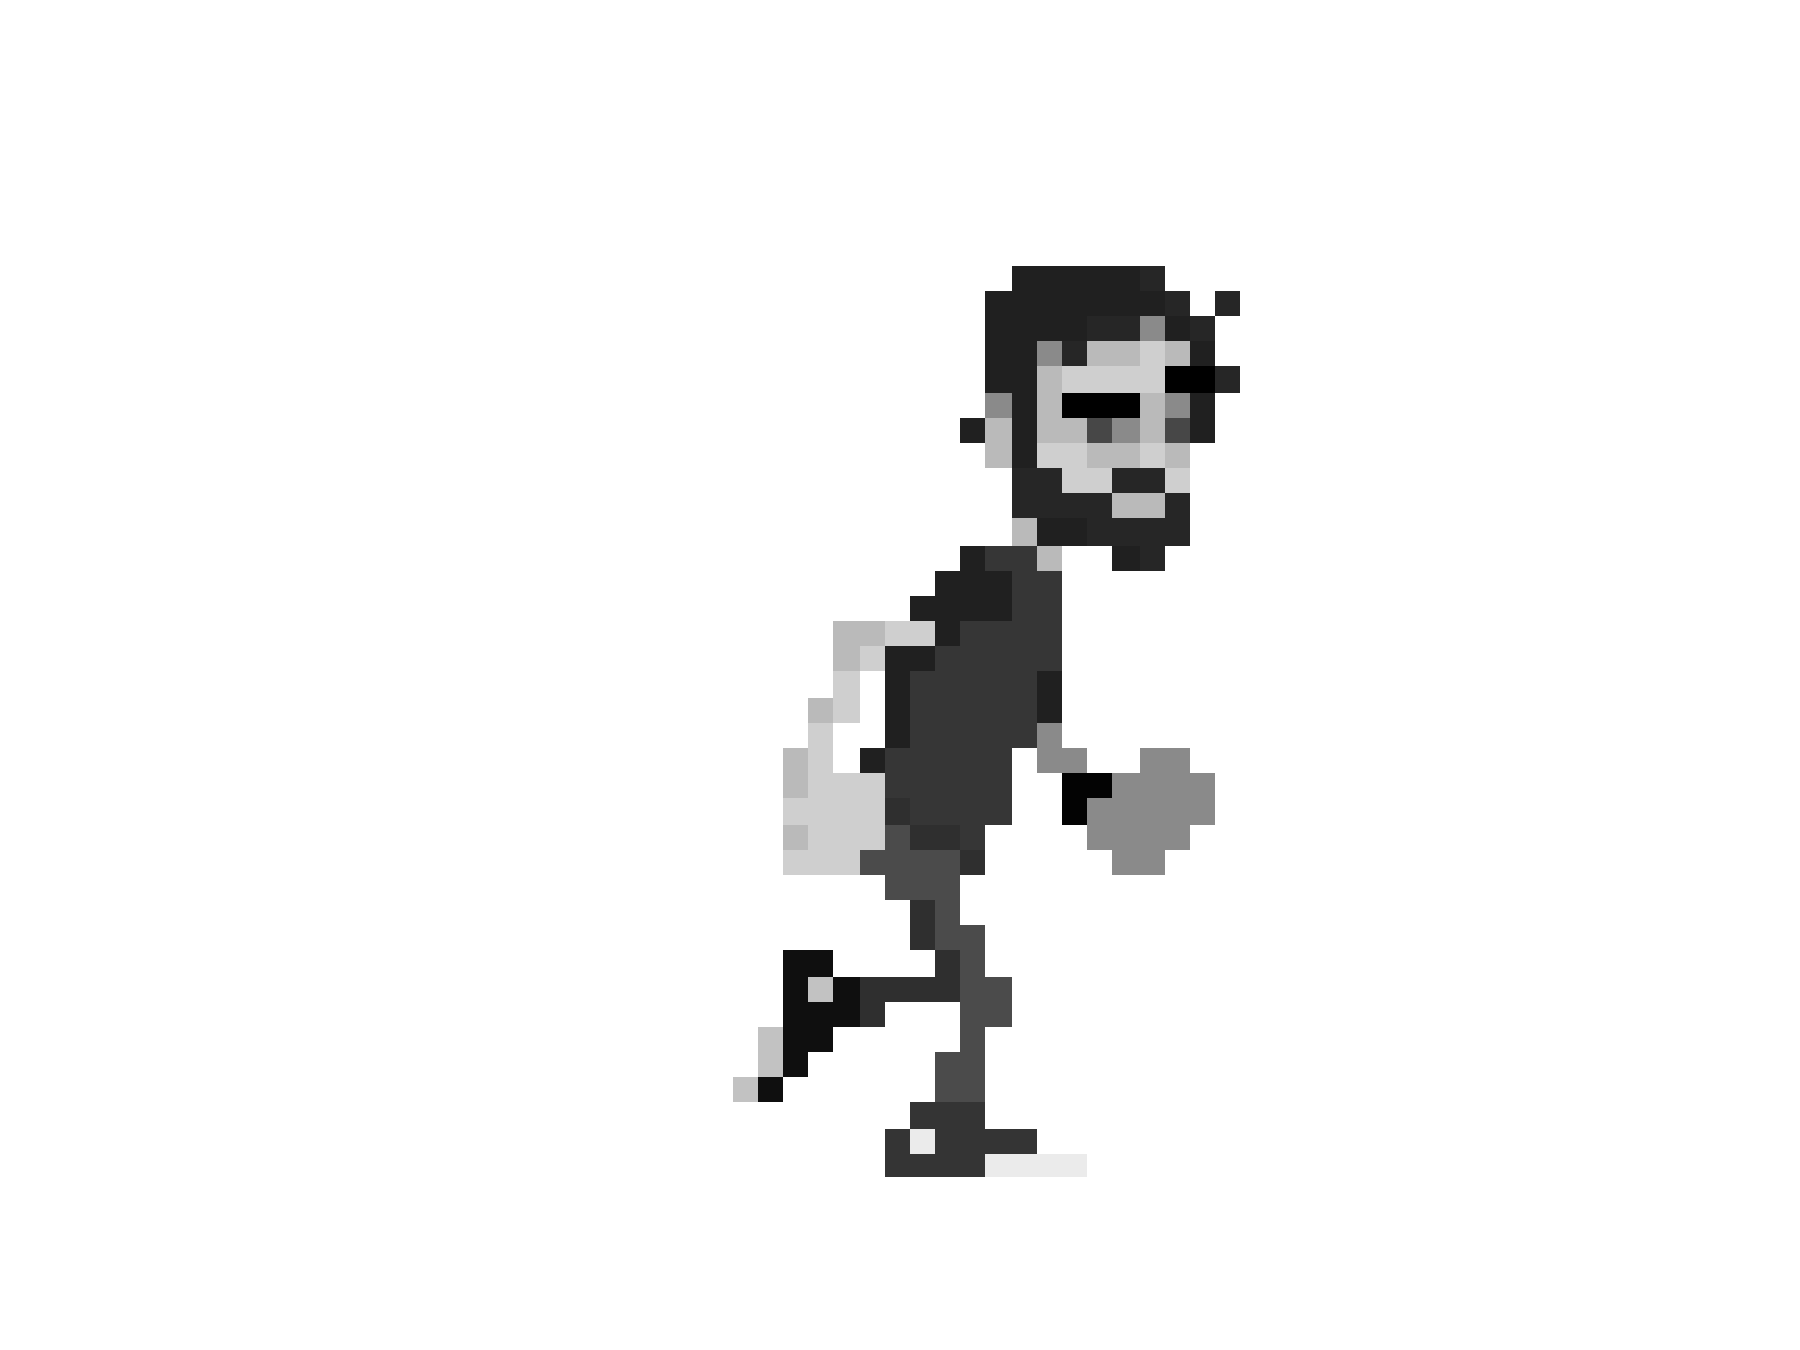
\includegraphics[width=0.5\textwidth]{./figures/origin.pdf}
    \hfill
    \caption{Origin}
    \label{fig1}
    \hfill
    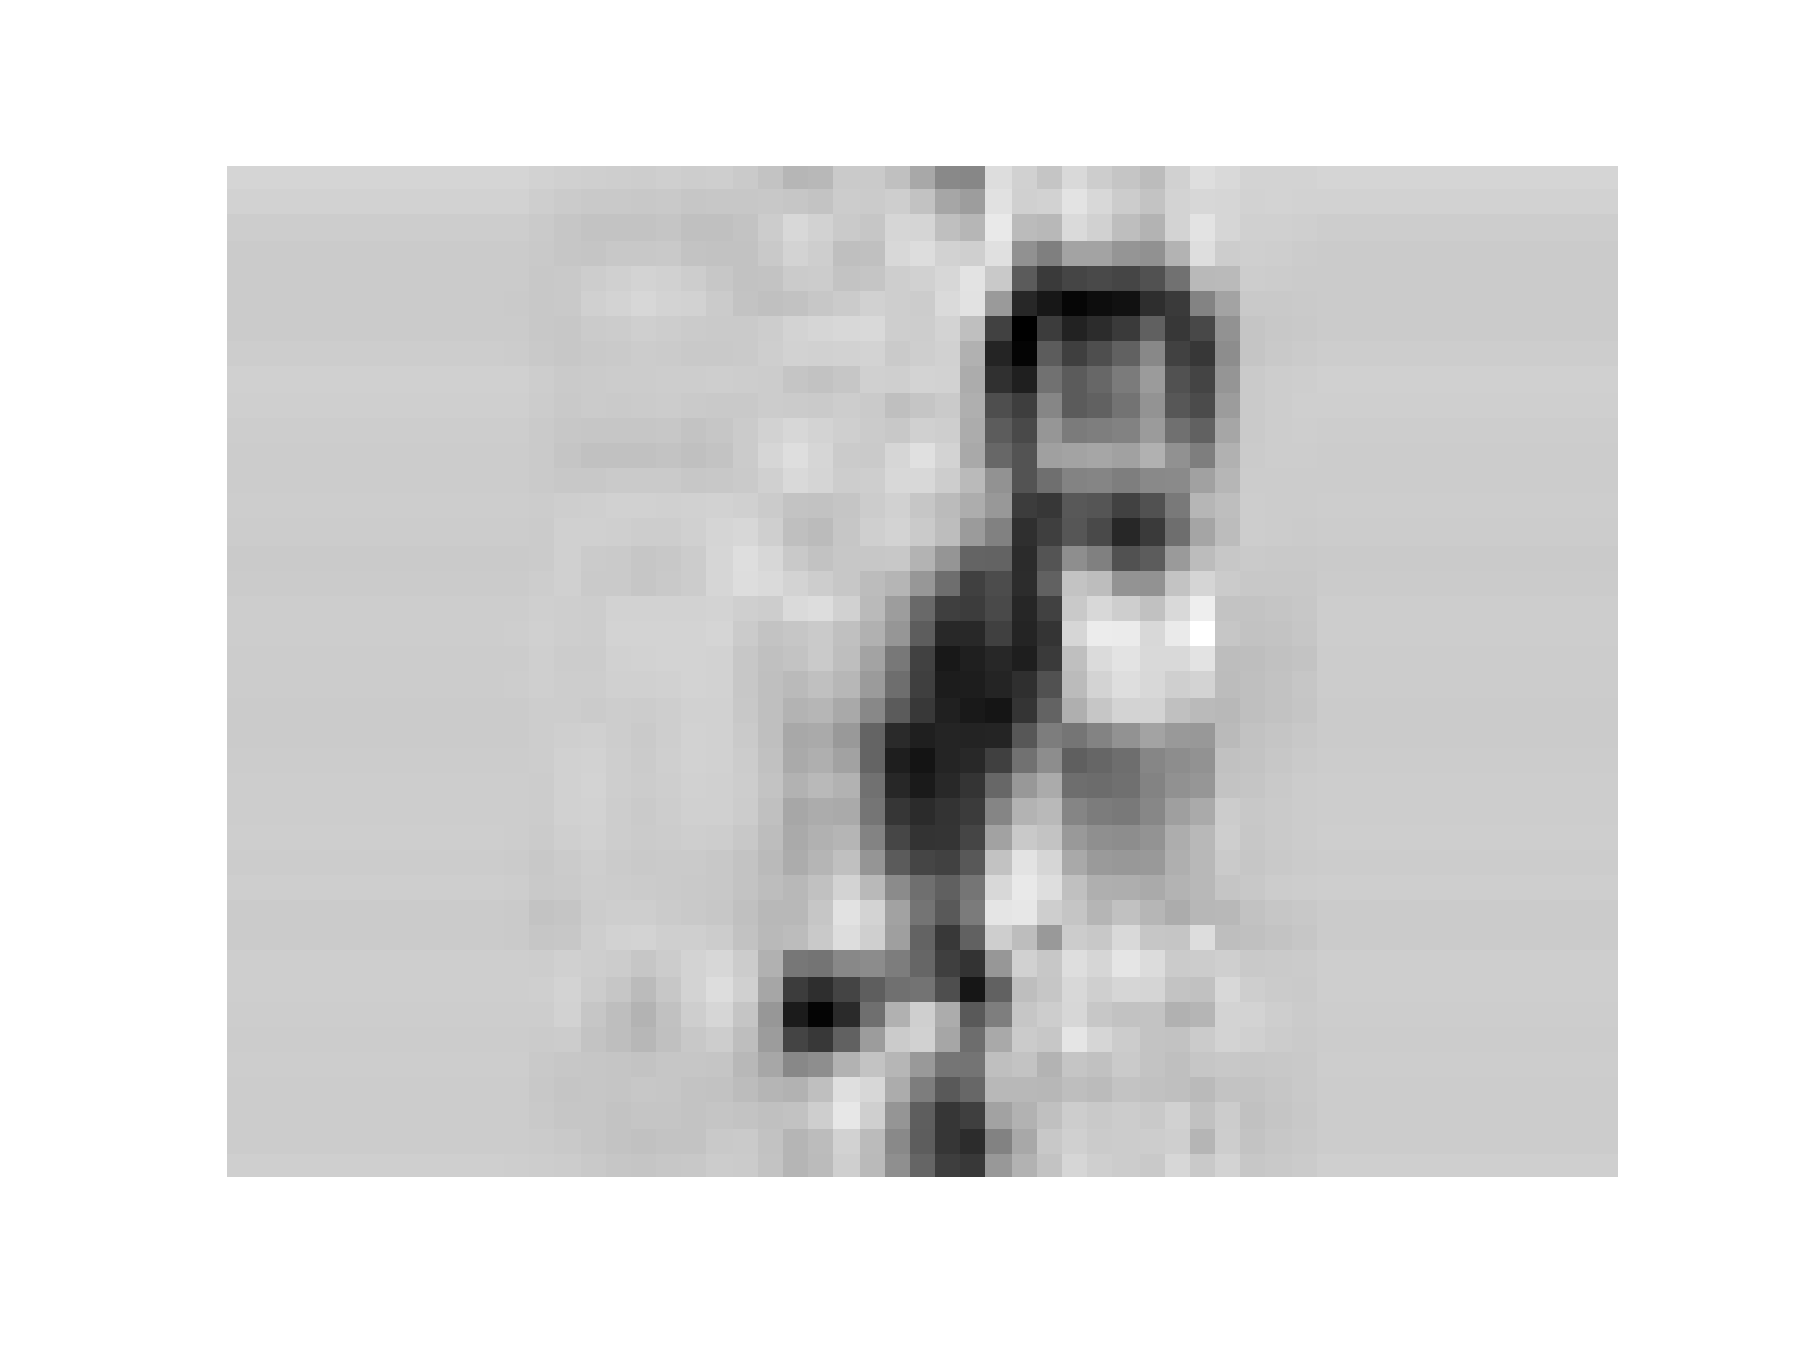
\includegraphics[width=0.5\textwidth]{./figures/approx.pdf}
    \hfill
    \caption{Approximated}
    \label{fig2}
  \end{multicols}
\end{figure}

Было взято gif-изображение размером $40 \times 55$ и состоящее из $12$ кадров. 
Далее продублировали сигнал $10$ раз, чтобы у нас был набор кадров из $10$ периодов. 

После этого применяется HOSVD с core-тензором размерностью $120 \times 10 \times 10$ и восстанавливается апроксимированный тензор. На $\ref{fig1}, \ref{fig2}$ изображены исходное и апроксимированное изображения. 
Из апроксимированного тезора составляется траекторная матрица картинок. 
В качестве звукового сигнала $Y$ используется синусойда с периодом в $12$ шагов:
\begin{gather*}
    Y = \left\{\sin\left(i * \frac{2 \pi}{12}\right) \right\}_{i=1}^{120}
\end{gather*}

К траекторным матрицам $U, V$, полученным из апроксимированного тензора $\underline{X}$ и $V$, применяется CCM. 
Берутся все точки $t \in \{2, \dots, 119\}$ и рассматриваются соседи $t^* \in \{t-1, t+1\}$.
Для них проверяется условие Липшица с $L=10^{-4}$. 
Было полученно, что все точки удовлетворяют условию Липшица. 
Поэтому можно утверждать, что имеется связи между звуковыми сигналом и апроксимированным рядом изображений. 

Проводились эксперименты с более "сильной" апроксимацией (core-тензор размера $12 \times 5 \times 5$). 
И также была обнаружена связь, что говорит о возможности применения этого метода для сильно сжатых рядов изображений. 
\end{document}